%!TEX root = Thesis_main.tex

\chapter{Control Theory}
\label{chapter3}

The interconnection between control theory and robotics has a history that of over half a century during which control theory has developed solutions problems in robotics field and problems in robotics have gained the new control theories. In the last decade or two, the Progress in robotic systems has been rapid, especially thinking about the applications increase, from machine tool industry to biomedical applications for example. The early design of robotic systems was to develop mechanisms to be as stiff as possible modeled as single-input/single-output (SISO) linear systems with each joint controlled independently. Then Point-to-point control used to perform simple tasks such as spot welding or pick and place operations. Encoureged by industry request, more complex tasks such as arc welding and spray painting has been enabled from Continuous-path tracking. But to consider more advanced tasks like assembly was restricted by the limited or nonexistent sensing of the external environment. Higher speeds and higher payload-to-weight ratios required a better understanding of modeling of nonlinear dynamical systems. For this reason new theoretical results in nonlinear, robust, and adaptive control enabled more advanced applications. Today, robot control systems are highly advanced with integrated sensing systems. Robot networks, surgical robots, mobile robots, underwater and flying robots, and others are starting to play important roles in society.
\section{PID Control}

PID architecture is the most common form of feedback controllers. The first implementation of PID controllers dates back to early 20th century. Today more than 90 \% of the control loops are PID type and are found in many areas. Nowdays is often combined with other advanced control techniques where generally the main usage of PID based controllers is for low level loops like motor controllers, integrated circuits etc. while advanced techniques are used for high level control.
When dealing with mobile robots, which are generally designed to perform tasks more or less autonomously, the aim of the controller can be manifold. In the case of mobile robots for pick and place operation the architecture of the online controller is generally hierarchic and the role of the PID regulator is to track desired high level control input.
\\ 
\\ The general control law for a PID controller is defined as follows: 

\begin{equation}
	p( t) = K_P e(t) +K_I\int\limits_{0}^{t} e(\tau)d\tau + K_D \frac{de(t)}{dt}
\end{equation}
The advantages of this basic control logic is the simplicity of implementation, lucid meaning, and the near-zero memory usage from the phisical hardware. Because of that and the many tuning techniques developed in years PID as been widely accepted in industry. Anyway this basic feedback control law present consisten limitation for andvanced applications. The goal of this type of controllers is to define a control law able to reduce the errors computed by means of the given measured data, so it works going after the real system measured outputs. The tuning of the controller is made chosing the parameters $K_P$, $K_I$ and $K_D$ that change the response of the closed loop system. Those parameters have to be chosen properly in order to achive stability and performances. Nevertheless, it's generally not possible to take into account any changes in the system dynamic. Because of that other control techniques have been developed in years.


\section{Inverse Dynamics Control}

The inverse dynamics control approach is directly related to the solution of the inverse dynamics problem of the system. Given the specified motion and the desired properties of the resulting system, the control inputs that ensure stability and realization of these control objectives are to be found. By appropriately inverting the dynamic model of the system to be controlled, a control law can be found. Generally this control law is chosen in order to cancel out the nonlinear part of the dynamics, to decouple the interactions between the regulated variables, and specify the behaviour of the convergence of the error. The inverse dynamics controller is able to enforce the execution of prescribed motion of the system and at the same time to control the interaction forces with the environment. If we consider a generic dynamical system in the form:
\begin{equation}
	H(q)\ddot{q}+C(q,\dot{q})\dot{q}+\tau_g(q)=\tau	
\end{equation}
The inverse dynamics control law can be defined: 
\begin{equation}
	\tau=H(q)v+C(q,\dot{q})\dot{q}+\tau_g(q)
\end{equation}
From this control law results that $\ddot{q}=v$. Where $v$ is a new conrol input, one approach to define it is with a PD (Proportional-Derivative) feedback:
\begin{equation}
	v = \ddot{q}_d+K_V\dot{e}_q+K_Pe_q
\end{equation}
The overall control input becomes:
\begin{equation}
	\tau=H(q)(\ddot{q}_d+K_V\dot{e}_q+K_Pe_q)+C(q,\dot{q})\dot{q}+\tau_g(q)
	\label{inverse_dyn_cont_law}
\end{equation}
So the resulting error dynamics is linear:
\begin{equation}
	\ddot{e}_q+K_V\dot{e}_q+K_Pe_q=0
\end{equation}
That is, properly choosing $K_V$ and $K_P$ parameters theconvergence of the error is zero.  
\\\
\begin{figure}
	\centering
	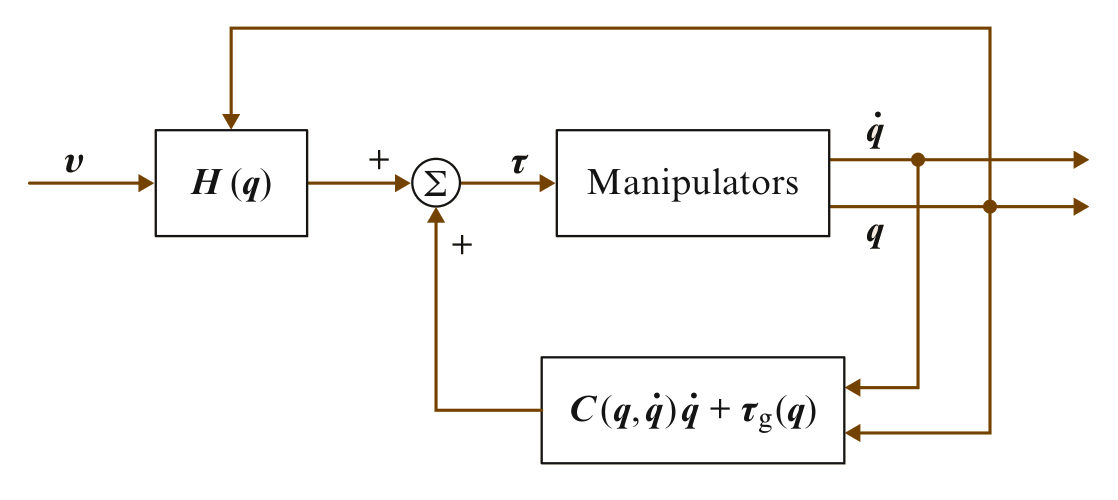
\includegraphics[scale=0.3]{torque_control}
	\label{Torque_control_scheme}
	\caption{Inverse dynamics control scheme}
\end{figure}
The usage of the inverse dynamics in Robot controller is widely diffuse and allows the to transform a MIMO nonlinear system into a simple decoupled linear system, nevertheless relies on a precise modeling of the dynamic system and a perfect knowledge of dynamical parameters. For those reasons classical inverse dynamics controllers are affected by changes in dynamical system properties more advanced techniques able to adapt to system modifications like adaptive control have been developed.  
\section{Adaptive Control}

Adaptive controller are different from other ordinary controller because the control parameters are time varying. Those parameters are adjusted by an online mechanism based on some signal of the closed-loop system. By means of this type of controller, it is possible to reach control goal even if the plant is subjected to uncertanties or modifications. There are many ways in which this controlled has been implemented, including adaptive computed-torque control, adaptive inertia-related control, adaptive control based on passivity, and adaptive control with desired
compensation. Adaptive computed-torque control will be presented as an example. Failures in model parameters estimation for classical torque control can lead to mismatch terms that can be interpreted as nonlinear perturbation.
We'll use the same approach of \ref{inverse_dyn_cont_law} but considering estimated parameters:
\begin{equation}
	\tau=\hat{H}(q)(\ddot{q}_d+K_V\dot{e}_q+K_Pe_q)+\hat{C}(q,\dot{q})\dot{q}+\hat{\tau_g}(q)
	\label{torque_control_estim}
\end{equation}
where $\hat{H},\hat{C},\hat{\tau}$ have the same functional form as $H,C,\tau_g$. By means of the properties of the dynamical model to be linear wih respect to the system parameters it is possible to write:
\begin{equation}
	hat{H}(q)\ddot{q}+\hat{C}(q,\dot{q})+\hat{\tau_g}(q)=Y(q,\dot{q}\ddot{q})\hat{a}
\end{equation}
where $Y(q,\dot{q}\ddot{q})$ is known as a regressor matrix and $a$ is the vector of the estimated parameters. Applying the control law defined as \ref{torque_control_estim} lead to:

\begin{equation}
	\hat{H}(q)(\ddot{e}_q+K_V\dot{e}_q+K_Pe_q)=Y(q,\dot{q}\ddot{q})\tilde{a}
\end{equation} 
where $\tilde{a}=\hat{a}-a$. Now under the assumption of $\ddot{q}$ measurable and non singularity of $\hat{H}(q)$ we rewrite the equation in state space form: 

\begin{equation}
	\begin{split}
		&\dot{x}=Ax+B\hat{H}^{-1}(q)Y(q,\dot{q}\ddot{q})\tilde{a} \\
		&\text{with} \quad x=[e_q^T,\dot{e}_q^T]^T \\
		&A=	\left[	
				\begin{matrix}
	 			0_n & I_n \\ -K_P & -K_V
				\end{matrix}
			\right],
			B=\left[	
				\begin{matrix}
	 			0_n \\ I_n
				\end{matrix}
			\right],
	\end{split}
\end{equation}
The new adaptive control law will then be: 
\begin{equation}
	\dot{\hat{a}}=-\Gamma^{-1}Y^T(q,\dot{q}\ddot{q})\hat{H}^{-1}(q)B^TPx
\end{equation}
where $\Gamma$ is a constant positive-definite matrix and $P$ is a symmetric positive-definite constant matrix that satisfy: 
\begin{equation*}
	PA+A^TP=-Q
\end{equation*} %  da aggiungere ref.
Q is a symmetric positive definite matrix with coherent dimension. The stability of the closed loop system and the boundedness of internal signals can be assessed studing the Lyapunov stability of the function $\dot{V}=-x^TQx$.  
For more details see \cite{craig1987adaptive}
\section{Optimal Control}

\begin{quote}
\textit{In place of determining the optimal sequence of decisions from the fixed state of the system, we wish
to determine the optimal decision to be made at any state of the system. Only if we know the latter, do
we understand the intrinsic structure of the solution.}
\emph{\begin{scriptsize}
Richard Bellman, Dynamic Programming,
1957. [Vinter, p. 435]
\end{scriptsize}}
\end{quote}

From a practical point of view, once the stability of a controller has been proved, nothing says that there is only one controller able to perform the control action. In other words since the stability proof doesn't determine a unique controller, generally it is possible to choose among different alternatives. It's pretty natural, in many contexts, that the choice of an optimal controller is preferred. The objective of optimal control theory, indeed, is to determine the control action that will cause a system to satisfy phisical constraints and at the same time to minimize (or maximize) some performance criterion. Generally the definition of this criterion (i.e. cost function) is done according with the application of the controller. Since there are many complex problems in control field that cannot be solved using classical techniques, optimal control theory has been studied and improved in 90's. At the same time, the increase in computation capability of calculators allows to implement those logics in many fields. However the design of an optimal controller generally relies on an exact model of the system. In fact, the presence of discrepancy between the model and the real system can lead to non-optimal solution that can easily end in an instable closed loop system. 
Let's consider a generic system described by nonlinear time-varying differential equation in $x\in R^n$:

\begin{equation}
	\dot{x}(t)=f(x,t)+G(x,t)u
\end{equation}
where $u \in R^m$ is the control input. We will consider the sistem without disturbancies term.
We will refer as an example to a quadratic optimal control problem. 
Every optimal controller needs the definition of a cost function, as example: 
\begin{equation}
	z=H(x,t)x+K(x,t)u
\end{equation}
such that: $H^T(x,t)K(x,t)=0, K^T(x,t)K(x,t)=R(x,t)>0$ and \\ $H^T(x,t)H(x,t)=Q(x,t)>0$. The quadratic cost function becomes:

\begin{equation*}
	\frac{1}{2}z^Tz=\frac{1}{2}x^TQ(x,t)x+\frac{1}{2}u^TR(x,t)u
\end{equation*}

The optimal control law with the quadratic cost function can be derived from  the solution of HJB (Hamilton-Jacobi-Bellman) equation for a positive-definite function $V(x,t)$ as in \cite{kirk1970optimal}.

\begin{equation}
	\begin{split}
		0&=HJB=(x,t;V)=V_t(x,t)+V_x(x,t)f(x,t) \\
		&-\frac{1}{2}		V_x(x,t)G(x,t)R^{-1 }		(x,t)G^T(x,t)V_x^T(x,t)+\frac{1}{2}Q(x,t)
\end{split}
\end{equation}

where $V_t=\frac{\partial V}{\partial t}$ and $V_x=\frac{\partial V}{\partial x^T}$. Then the inverse quadratic optimal control problem is to find a set $Q(x,t)$ and $R(x,t)$ for which $V(x,t)$ is a solution for the HJB. That defines the oprimal controller such as:

\begin{equation}
	u=-R^{-1}(x,t)G^T(x,t)V_x^T(x,t) 
\end{equation}

Since in most application it is required to design a controller able to generate control inputs starting from observation of system outputs, there are three alternatives: 

\begin{enumerate}
\item Design the controller in closed loop form and by means of a computational unit solve optimal control problem on-line
\item Precompute an optimal control law offline and then synthetize it into a special-purpouse digigtal controller.
\item Use a suboptimal controller whose parameters have been defined offline. 
\end{enumerate}

Anyway generally speaking the proper choice is made according to the application. The system evolution frequency for example gives many limitation to on-line solution of the optimal control problem. 
A typical implementation of optimal control theory is made in practice by means of Model Predictive Control. 

\section{Model Predictive Control}

\epigraph{\textit{Discrete Dynamic Optimization Applied to On-line Optimal Control}}{\begin{scriptsize}
Rafal, Stevens, AiChE Journal, 1968
\end{scriptsize}}

The term Model Predictive Control (MPC from now on) designate a wide range of control strategies which use explicitly the model of the system to obtan the control action minimizing a specific cost function. The first development originated in the late seventies with IDCOM (Identification and Command) logic. Using impulse response for the plant model and optimiziang a quadratic objective function, This control, settled the basis of an architecture that has been developed considerably since then, expecially over the last two decades both within research community and industry.
Such a succes is probably due to it's generality, in fact MPC formulation can be considered as one of the most general ways to pose a process control problem. It's formulation can integrate optimal control, stochastic control, control of processes with dead time and multivariable control. In general nonlinear processes which are frequently found in industry, can be handled by MPC logics. Futhermore , unless stability and robustness proof is difficult to asses because of the finite horizon, it has been found to be quite robust in many applications. Anyway, although both in industry and in research is widely diffuse, MPC has not yet reached the potential it suggest. One reason can be found in the fact that requires mathematical knowledge which is not usually available by control engineers in practice. This control architecture is generally an open framework that allows the development of many applications in use at the current
time, not only in the industrial processes but also application to robotics, power plants, PVC plants, servos etc. Since MPC showed good performances in many of these applications as well as it's ability to operate whit few intervention for long periods of time, the interest in this control strategy is increasend in the last decades. This can be justified also by the increased capability in solving complex problem, sometimes complex rather than nonlinear. Many are the advantages with respect to other control techniques: \\

\begin{itemize}
\item Tuning is relatively easy.
\item Implementing simple dynamics to more complex ones, it can be used to control a great variety of processes also including delay times, nonminimum phase or unstable systems.
\item It can introduce feed forward control to compensate measurable disturbances.
\item Easily defined for multivariable problems.
\item Can be easily extended to treat the constraints and these can be systematically included during the design process.
\item It is very useful when future references are
known for example for robotic applications.
\item It is an open methodology with many applications allowing further extensions.
\end{itemize}


Nevertheless it also has its drawbacks. First of all is that it's derivation is more complex than the one of classical PID controllers. Then, even if with a good model of the system we can prederivate the controller, the system can usually be subject to modification in it's dynamics, so the derivation needs to be done online, increasing significantly the computational effort. Moreover the introduction of constraints generally increase the computational time of the problem, that may result in a low frequency controller, not suitable for some applications.
But computational time is not the only drawback. To be able to perform correctly, the system needs to be accurately modeled and that may not be possible in some cases in which for example the system is very complex or higly coupled.
Even if there are many practical problems in implementing MPC for complex or high frequency control problems, it is a control logic suitable for many applications in which perform nicely. 
\begin{table}
	\centering
	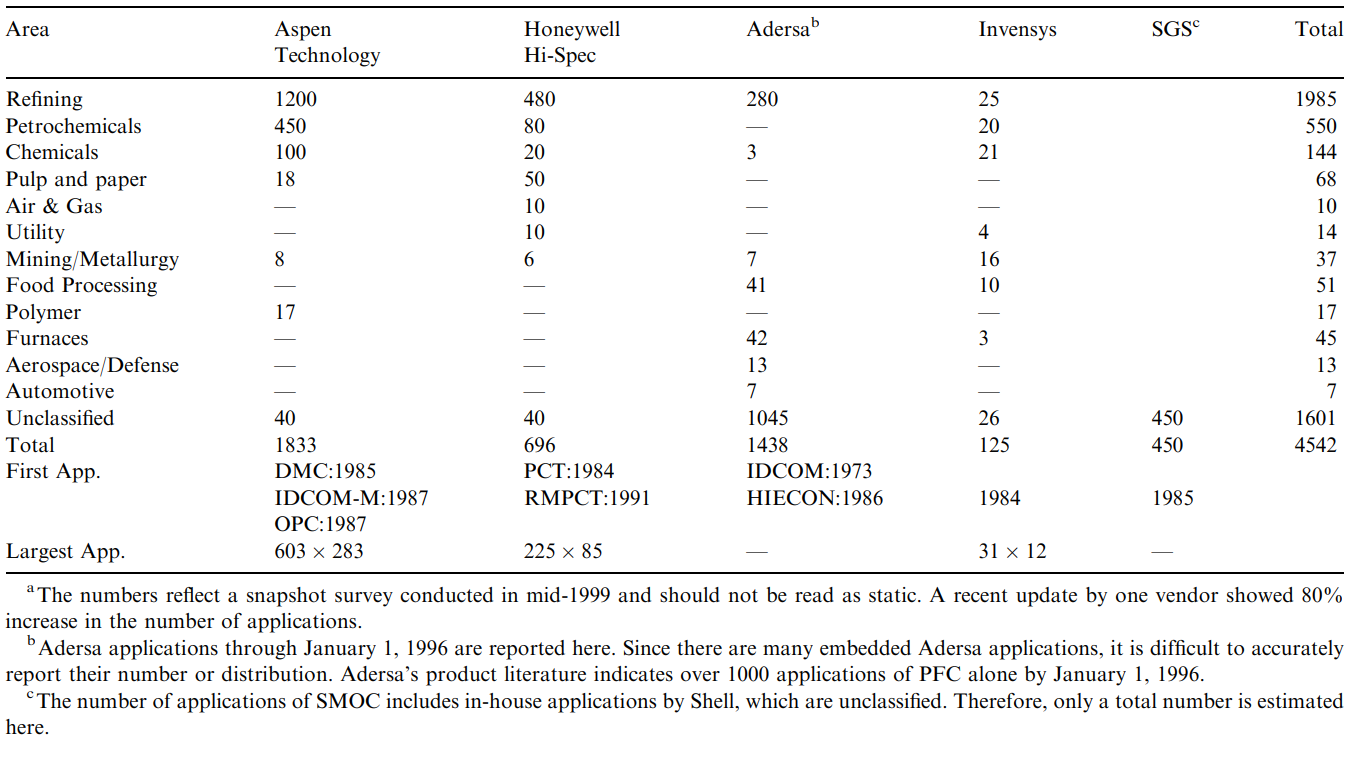
\includegraphics[scale=0.28]{mpc_usage_table}
	\caption{Summary of linear MPC applications by areas}
	\label{mpc_usage_table}
\end{table}

In \cite{qin2003survey} is presented an overview of commercially available model predictive control technology, both linear and
nonlinear. The table \ref{mpc_usage_table} from that work shows the applications of MPC logic by area. Such a diffuse usage of this control logic collocate MPC as the second most used control methodology after PID. In the last decades MPC has been investigated in may fields as Process control (linear or nonlinear MPC), Automotive (Explicit, Hybrid MPC), Aerospace(LTV MPC), ICT(distributed/decentralized MPC), Energy or Finance (stochastic MPC).
As most of the drawbacks are related to the model identification or optimization algorithms capability, fields in which research is working nowdays, MPC is still of high importance for research and industry.
In this section basic concepts of Model Predictive Control will be presented in order to understand more in detail what we developed. More details in MPC theory can be found in \cite{camacho2013model}

\subsection{Basic Concepts}

As mentioned before Model Predictive Control use the model of the system and the definition a customized cost function in order to set and solve an optimization problem to find the correct control inputs to perform a specific control task.
A diagram of how MPC basic architecture is schematized below: \\
 
\begin{figure}[h!]
	\centering
	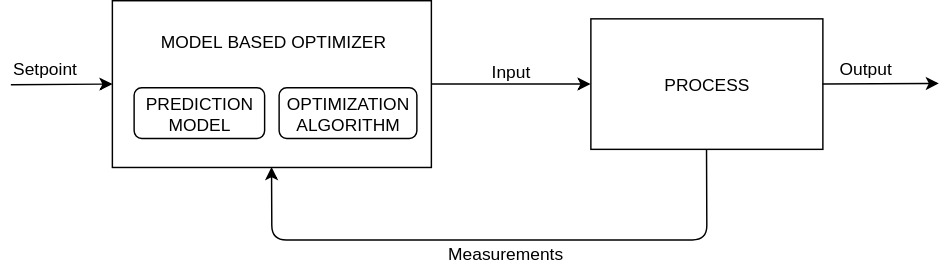
\includegraphics[scale=0.4]{MPC_base_diagram}
	\caption{MPC basic architecture scheme}
	\label{mpc_base_diagram}
\end{figure}
The model based optimizer (usually a computer) use optimization algorithms in accordance with the model of the system and given measures to minimize the cost function which is generally dependent on the error with respect to the given setpoint. Generally other constraints can be added to the problem in order for example to keep the states variables within feasible ranges. The output of the computation is then the input of the real process to be controlled. In  practice the solution of the problem usually has two main limitation:

\begin{itemize}
\item Model of the process: the nature of the MPC is based on the possibility to forecast the future output of the system by means of a model. Because of that, to have a reliable prediction, we need the system model to be accurate.

\item Optimization algoritm: as mentioned before, the more the system is complex and constraints are added to the problem, the more the problem will be computationally heavy. A proper optimization algoritm needs to be choose in accordance with the application of the controller.
  
\end{itemize}
Any controller belonging to MPC family is usually amenable to the following methodology:
\begin{figure}[h!]
	\centering
	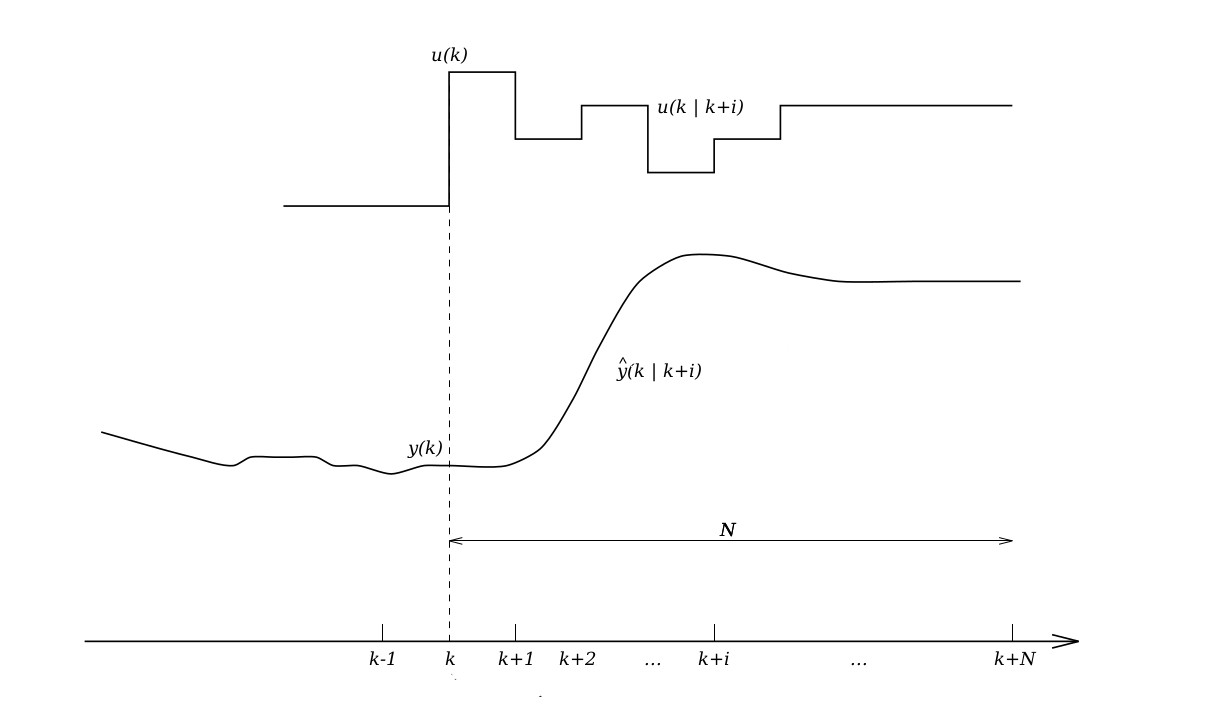
\includegraphics[scale=0.32]{mpc_horizon_base_scheme}
	\caption{MPC strategy}
	\label{mpc_horizon_base_scheme}
\end{figure}

\begin{enumerate}
\item Future outputs defined on a prediction horizon $N$ as $\hat{y}(k|k+i)$ for $i=1\ ...\ N-1$ are predicted starting from past inputs and outputs as a function of the future control actions $u(k|k+i)$, $i=0\ ...\ N-1$.
\item The future control signal set is calculeted optimizing a given cost function to keep the predicted future output as close as possible to the given reference trajectory $y_d(k+i)$. The objective function is generally defined as a quadratic fuction with respect to this reference trajectory. Control effort term is also usually added to the cost in most cases. If the system is linear and the cost function is quadratic with respect to the error then an explicit solution can be found, otherwise merical methods have to be used instead.
\item The computed control action $u(k|k)$ is applied to the process then another optimization problem is set based on new measures in order to find $u(k+1|k+1)$ that will be in principle different from $u(k|k+1)$. 
\end{enumerate}
The sequence above repeats continuously following the so called Reciding Horizon principle. In order to be implemented, the model based optimizer, is designed following this scheme: \\
\begin{figure}[h!]
	\centering
	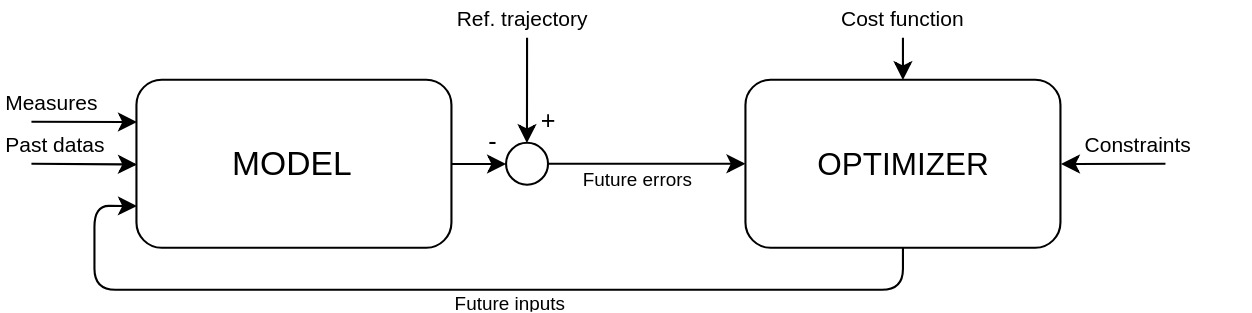
\includegraphics[scale=0.32]{scheme_model_based_opt}
	\caption{Model based optimizer}
	\label{scheme_model_based_opt}
\end{figure}
\\
The definition of prediction model can be done in several ways like inpulse response, step response, transfer function, state space and more complex representation like neural networks for nonlinear systems. We will refer to the state space representation for the prediction model as it is easy to implement and to integrate.

Let's define the discrete linear time invariant (LTI) model of the process in state space form as:

\begin{equation} \label{system_evolution}
	\begin{split}
		\begin{cases}
			x_{k+1}&=Ax_k+Bu_k \\
			y_{k+1}&=Cx_k
		\end{cases}
	\end{split}
\end{equation}

where $x \in R^{n_x}$ is the state, $y \in R^{n_y}$ and $u \in R^m$ are respectively the output and the control action and $A$, $B$ and $C$ are the matrices of the system. The prediction of the output for this model is given then by:

\begin{equation}\label{system_prediction}
	\hat{y}(k\ |\ k+i)=C\hat{x}(k\ |\ k+i)=C\left[A^i x(k) + \sum_{j=1}^{i} A^{j-1}Bu(k\ |\ k+i-j)\right]
\end{equation}

which can be defined in matrix form as: 
\begin{equation}
\begin{split}
	\left[ \begin{matrix} \hat{x}_k(1) \\ \hat{x}_k(2) \\ \vdots \\ \hat{x}_k(N) \end{matrix} \right] = \underbrace{\left[ \begin{matrix}
	CB		 & 	0	    &	\dots	&	0 		\\
	CAB		 & 	CB	    &	\dots	&	0 		\\
	\vdots	 &  \vdots  &	\ddots	&	\vdots	\\
	CA^{N-1}B & CA^{N-2}B &   \dots   &	CB			
	\end{matrix}\right]}_{\bar{H}}\left[ \begin{matrix} u_k(0) \\ u_k(1) \\ \vdots \\ u_k(N) \end{matrix} \right]+ \underbrace{\left[ \begin{matrix} CA \\ CA^2 \\ \vdots \\ CA^N \end{matrix} \right]}_{\bar{T}}
	\end{split}	
\end{equation}

The definition of the cost function has a strong influence on stability proof as well as the convergence of numerical optimization methods. A preferrable choice is to consider a positive definite function of the error with respect to the reference trajecotry. As the problem can be easily moved a zero-reference problem we will refere to that case. For simplicity of notation we will refer to $\hat{y}(k\ |\ k+i)$ as $\hat{y}_{k|i}$
\begin{equation} \label{costfunction}
	\begin{split}
		J(x_{k|0},\textbf{u}_k) = \sum_{i=0}^{N-1} \left[\hat{y}_{k|i}^T Q \hat{y}_{k|i} + u_{k|i}^TRu_{k|i} \right] + \hat{y}_{k|N}^T P \hat{y}_{k|N}
	\end{split}	
\end{equation}

where $\textbf{u} \in R^{mXN}$ with $\textbf{u} = [u_{k|1}\ u_{k|2}\ ...\ u_{k|N-1}]$ is the control action that has to be found for the predicted horizon. R, Q and P are positive definite weight matrices. Let's write the cost function in matrix form: 

\begin{equation*}
\begin{split}
		J(x_{k|0},\textbf{u})&=x_{k|0}^T Q x_{k|0} + 
		\left[ \begin{matrix} \hat{x}_{k|1} \\ x_{k|2} \\ \vdots \\ \hat{x}_{k|N} 		\end{matrix} \right]^T \underbrace{\left[ \begin{matrix} 
Q	 		&		 0	  	&  	0	  &  \dots  &  0 \\ 
0 			&  	 Q 	  	& 		0 	  &  \dots  &  0 \\
\vdots  	& 	  \vdots  	&   \ddots   &  \vdots &  0 \\
0 			& 	  \dots  	&      0     &      Q  &  0 \\
0			& 		 0 		&	  \dots   &      0  &  Q
\end{matrix} \right]}_{\bar{Q}}
\left[ \begin{matrix} \hat{x}_{k|1} \\ x_{k|2} \\ \vdots \\ \hat{x}_{k|N} \end{matrix} \right] +  \\ 
&+\left[ \begin{matrix} u_{k|0} \\ u_{k|1} \\ \vdots \\ u_{k|N-1} 		\end{matrix} \right]^T \underbrace{\left[ \begin{matrix} 
R	 		&		 0	  	&     \dots   &  0 \\ 
0 			&  	     R 	  	&     \dots	  &  0 \\
\vdots  	& 	  \vdots  	&    \ddots   &  \vdots \\
0			& 	  \dots     &        0    &  R
\end{matrix} \right]}_{\bar{R}}
\left[ \begin{matrix} u_{k|0} \\ u_{k|1} \\ \vdots \\ u_{k|N-1}  \end{matrix} \right] 
\end{split}
\end{equation*}

Substituting the \ref{system_prediction} we obtain:

\begin{equation}\label{costfunction_expr}
\begin{split} 
 J(x_{k|0},\textbf{u}_k)&=x_{k|0}^T Q x_{k|0} + (\bar{S}\textbf{u}_k+\bar{T}x_{k|0})^T\bar{Q}(\bar{S}\textbf{u}_k+\bar{T}x_{k|0}) + \textbf{u}_k^T\bar{R}\textbf{u}_k \\ 
 &= \frac{1}{2}\textbf{u}_k^T \underbrace{2(\bar{R}+\bar{S}^T\bar{Q}\bar{S})}_{H}\textbf{u}_k + x_{k|0}^T\underbrace{2\bar{T}^T\bar{Q}\bar{S}}_{F}\textbf{u}_k+\frac{1}{2}x_{k|0}\underbrace{2(Q+\bar{T}^T\bar{Q}\bar{T})}_{Y}x_{k|0} \\
 &=\frac{1}{2}\textbf{u}_k^TH\textbf{u}_k+x_{k|0}F\textbf{u}_k+\frac{1}{2}x_{k|0}Yx_{k|0}
 \end{split}
\end{equation}
Once we have express the cost as a function of the measured initial state $x_k(0)$ and the future control action we can perform the optimization by zeroing the gradient:
\begin{equation}
	\nabla_{\textbf{u}_k}J(x_{k|0},\textbf{u}_k)=H\textbf{u}_k+F^Tx_{k|0}=0
\end{equation}
\label{grad_obj_fun}
$\textbf{u}_k$ is then derived inverting the \ref{grad_obj_fun}:
\begin{equation*}\label{MPC_control_law}
	\textbf{u}_k= \left[
	\begin{matrix}
			u_{k|0} \\ u_{k|1} \\ u_{k|2} \\ \vdots \\ u_{k|N-1}
	\end{matrix}\right] = -H^{-1}F^Tx_{k|0}
\end{equation*} 

The contorl law generated that can be derivated is then:
\begin{equation}
u(t)=-\left[\ I\ 0\ \dots\  0\ \right]H^{-1}Fx(t)\triangleq Kx(t)
\end{equation}
The same result can be obtained from DARE (discrete-time Algebraic Riccati Equation) as done in \cite{magni2006complementi}.
By means of this result it is possible to implement the MPC with a simple feedback loop. Since it is possible, the derivation of \ref{MPC_control_law} is done offline in this case, the online controller will then be fast given that the computational effort depend almost only on the inversion of $H$. 
Anyway the assuptions of Linear and time invariant system are considerably strong, many of practical systems present nonlinearities an time varying relationship. Because of that, different ways to minimize the \ref{costfunction_expr} have to be found.
Usually what is done in practice is to use algorithms to perform numerical optimization to find an approximation of the optimal solution. The main issue in the solution of the optimization problem is related to the well-definiteness of the problem. Indeed the correct choice of objective function form has to be done. usually the quadratic form allows to define convex problems in order to guarantee the unicity of the solution.

\subsection{Constraints}

In order to take into account feasibility sets and to gurantee stability, constraints are usually added to the optimization problem that becomes: 

\begin{equation} \label{MPC_problem_constrained}
\begin{split}
		&\qquad min_{\textbf{u}_k}\ J(x_{k|0},\textbf{u}_k) \\
		\textnormal{where}\ \  
		 J(x_{k|0},\textbf{u}_k) &= \sum_{i=0}^{N-1} \left[\hat{y}_{k|i}^T Q \hat{y}_{k|i} + u_{k|i}^TRu_{k|i} \right] + \hat{y}_{k|N}^T P \hat{y}_{k|N} \\
		\textnormal{respecting}\ &  	
		\begin{cases}
			\hat{x}_{k+1}&=A\hat{x}_k+Bu_k \\
			\hat{y}_{k+1}&=C\hat{x}_k
		\end{cases} \\
		\textnormal{s.t.}\qquad
		&\ \ \ \ 0 \leq f(x)\leq 0 \\
		&\ \ \ \ 0 \leq g(u)\leq 0 \\
	\end{split}	
\end{equation}

This notation allows us to introduce both equality and inequality constraints. In paractice the constraints are divided into: 
\begin{itemize}
 \item \textbf{Input constraints}: generally represent philical limitation for the control $\textbf{u}_k$ and are defined as "hard" constraints.
 	\item \textbf{State/Output constraints}: usually come from rescrictions into the operational space, they can both be "soft" or "hard".
\end{itemize} 

Hard constraints on the state or on the output gives generally complication in the implementation but soft constraints have to be defined properly according to the application. Moreover constraints allows a resonable control action to be generated when measured or estimated states moves outside the feasible sets. Given this outline, many are the possible constraints definition: Band Constraints, Overshoot Constraints, Monotonic Behaviour, Nonminimum Phase Behaviour, Actuator Nonlinearities, Terminal State Equality Constraints, Terminal Set Constraints and more. Given that it is possible to define different constraints we will refer to terminal state equality constraint as it will be useful for the stability proof later on. \\
The terminal state constraint is basically defined as: 

\begin{equation}
\hat{y}_{k|N}=C\left[A^i x_{k|0} + \sum_{j=1}^{i} A^{j-1}Bu_{k|k+N-j}\right]=\bar{y}_N
\end{equation}
that can be rewritten following the form in \ref{MPC_problem_constrained}: 
\begin{equation}
0 \leq \hat{y}_{k|N}-\bar{y}_N \leq 0
\end{equation} 

\subsection{Stability and Feasibility}

In this section stability and feasibility of MPC are investigated in order to give a clear understanding of what done to proof stability of the MPC we developed. To assess feasibility we need to investigate and proff is the problem have a solution and then to proof recursive feasibility, so the system accept a solution $\forall\  t>0$. As well as feasibility, stability has to be proof in order to have convergence of the performed trajecotry. We will refer to a regulation problem, so the set point will be defined as the origin.
The set $X_{k}$ of initial states $x_{k|0}$ defined for any instant $k$ that ensure feasibility for the MPC problem \ref{MPC_problem_constrained} is defined as:

\begin{equation}
	\begin{split}
		X_{k}=\lbrace\ x_{k|0}\in\mathbb{R}^n\ |\ \exists\  (u_{k|0}, \dots , u_{k|N-1})\ \textnormal{s.t.}\ x_{k|i} \in X, u_{k|i} \in U,\ &  \\ 
		\forall\  i=0,\dots,N-1,\ x_{k|N} \in X_f\ \rbrace& \\ 
	\end{split}
\end{equation}
where $U$ is the region of the control action, $X_f$ is the region of terminal states and $x_{k|i+1}$ is propagated following the \ref{system_evolution}
 The feasible and unfeasible points in a regulation problem can be visualized on a graph (see \ref{feasibility_image1}) and a region of feasible points can be defined (see \ref{feasibility_region})

 \begin{figure}%
\centering
\subfigure[Feasibility points]{%
\label{feasibility_image1}%
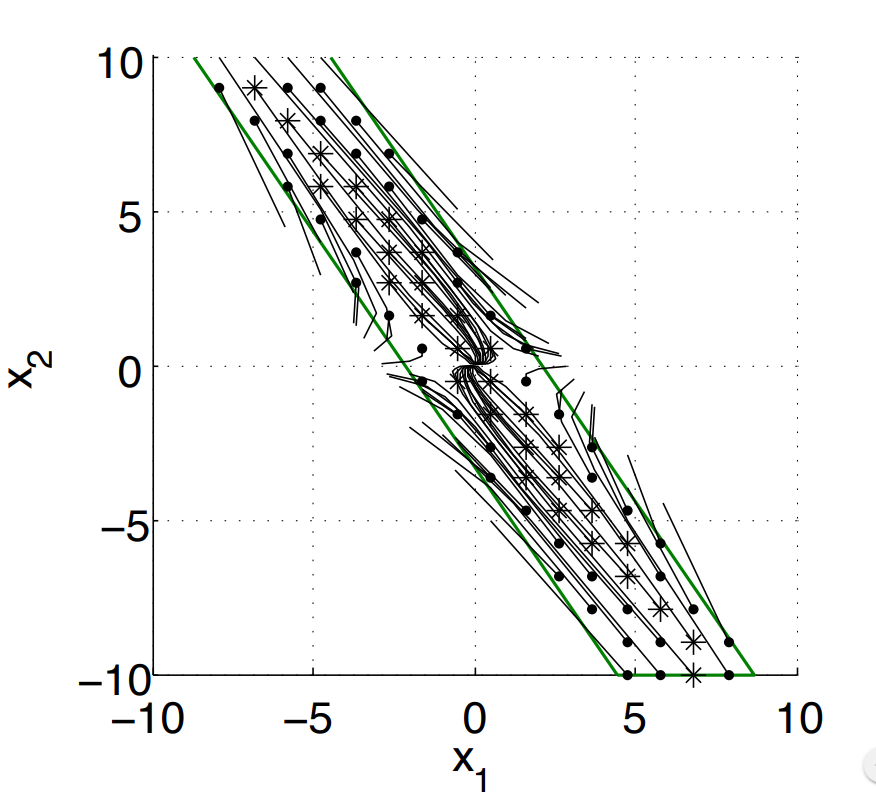
\includegraphics[scale=0.2]{feasibility_image1}}%
\qquad
\subfigure[Feasibility region]{%
\label{feasibility_region}%
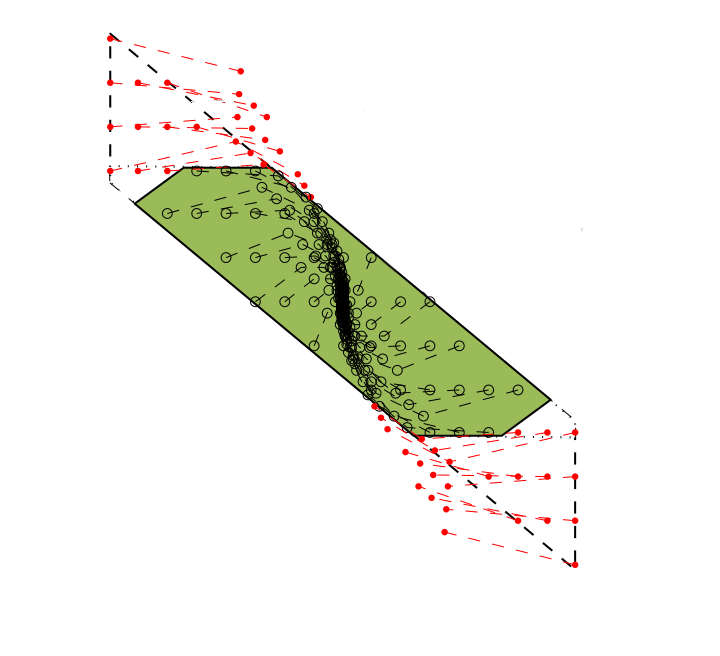
\includegraphics[scale=0.25]{feasibility_region}}%
\caption{Feasibility set}
\end{figure}

 Feasibility of a point does not guarantee the feasibility of the following inputs generated by the control action. Because of that Recursive feasibility has to be assessed. That means to show that:
 \begin{equation}
 \begin{split}
  &\ \ \ \ \ \ \ \ \ \forall\ k\ \exists\  \textbf{u}_k\in U\  \textnormal{s.t. } \\ 
  \textnormal{given } &x_{k|0} \in X, \  x_{k|i} \in X\  \forall\ i = 1,\  \dots\ , N-1   
 \end{split}
 \end{equation}
\begin{figure}[h!]
	\centering
	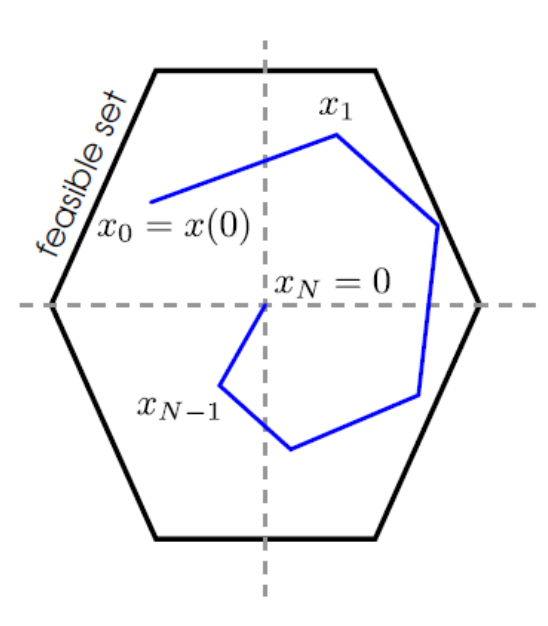
\includegraphics[scale=0.27]{feasible_image2}
	\caption{Recursive feasibility}
	\label{feasible_image2}
\end{figure}

While feasibility proof is straightforward because it is only affected by outputs hard constraints, stability is difficult to assess in some cases.
Stability is a complex function of $N, Q, R, P, U$ and admissible outputs of the system.
Usually the stability proof of the MPC is verified imposing terminal constraints and weigths on the terminal state. There are many well studied stability proofs for MPC problems:

\begin{itemize}
\item Infinite horizon MPC (N = $\inf$) with no additional constraints
\item Terminal point constraints ($x_{k|N}=0$)
\item Relaxed terminal constraints ($x_{k|N} \in X_f $)
\end{itemize}

The equilibrium point of a controlled system is said to be Lyapunof stable in $X$ if $\forall k \in \mathbb{N}$
\begin{equation}
\begin{split}
\forall&\ \epsilon > 0, \exists\ \delta(\epsilon) >0 \textnormal{ such that } \forall x_{k|0} \in X : \\
&||x_{k|0}|| \leq \delta(\epsilon) \implies ||x_{k|i}|| < \epsilon \forall\ i \in \mathbb{N}
\end{split}
\end{equation}

Stability proof is generally made by showing that the cost function to be minimized is a Lyapunov Function and admits an equilibrium point in the origin (regulation problem). The if $J$ is a Lyapunov function, the equilibrium point is stable with region of attraction $X$.

A function $V:X\rightarrow\ \mathbb{R}_+$ is a Lyapunov function if $\forall\ x \in\ X$:
\begin{equation} \label{Lyap_func}
\begin{split}
	V(x)>0 \rightarrow& \forall\ x \neq 0 \\
	V(0)=&\ 0 \\
	V(x_{k+1})-V(&x_{k}) \leq 0
\end{split}
\end{equation}

In order to guarantee convergence, asymptotic stability in $X$ of the equilibrium point has also to be verified. Hence it's needed to verify that it is Lyapunov stable and attractive in $X$ ( $\lim_{k \to \infty}||x_k||=0\ \forall\ x\ \in\ X$ ). 
That can be verified by extending the \ref{Lyap_func} asking: 
\begin{equation}
	V(x_{k+1})-V(x_{k}) < 0
\end{equation} 
\\ 
\\
Now let's consider for simplicity the cas in which $C=I$ so the system in \ref{system_evolution}becomes:
\begin{equation*}
x_{k+1}=Ax_k+Bu_k
\end{equation*}

We will assess stability by means of terminal constraints imposition (i.e. $x_{k|N}=0$) considering the quadratic cost function in \ref{costfunction} with  $J(x_{k|0},\textbf{u}_k)=J_k(x_0,\textbf{u})$
\begin{equation}
\begin{split}
J_k(x_0,\textbf{u}) &= \sum_{i=0}^{N-1} \underbrace{\left[x_{k|i}^T Q x_{k|i} + u_{k|i}^TRu_{k|i} \right]}_{q(x_i,u_i)} +\ \underbrace{x_{k|N}^T P x_{k|N}}_{p(x_N)} \\
\textnormal{and}\ \  x_n&=0
\end{split}
\end{equation}

Recursive feasibility has first to be verified:
Assuming the feasibility of the point $x_0$ and defining $[u_0^*,\ u_1^*,\ \dots,\ u_{N-1}^*]$ the optimal control sequence computed minimizing $J_0(x_0,\textbf{u})$, following the MPC strategy we apply $u_0^*$. The evolution of the system will then be $x_1=Ax_0+Bu_0^*$.
Now at instant $k=1$ the control sequence $[u_0^*,\ u_1^*,\ \dots,\ u_{N-1}^*,\ 0]$ is feasible because applying a null control input and given that $x_N=0$ the resulting final state is $x_N+1=0$. This implies that, in presence of end point constraints, the recursive feasibility is verified assuming $x_0$ feasible.

Once feasibility has been assessed, stability has to be investigated by checking if $J$ is a Lyapunov function. So, since we are interested in asymptotic stability, we need to verify;

\begin{equation}
J_0^*(x_1)<J_0^*(x_0)\ \ \ \forall x_0 \neq 0
\end{equation}

Follows that:
\begin{equation}
	\begin{split}
		&J_0^*(x_0)= \underset{=0}{\cancel{p(x_N)}}+\sum_{i=0}^{N-1} q(x_i,u_i^*) \\
		&J_0^*(x_1) \leq \tilde{J}_0(x_1)=\sum_{i=1}^{N}q(x_i,u_i^*) \\
		 = \sum_{i=1}^{N-1}&q(x_1,u_i^*)-q(x_0,u_0^*)+q(x_N,u_N) \\
		 &\ =\  J_0^*(x_0)-q(x_0,u_0^*)+\underset{=0}{\cancel{q(0,0)}} \\
	\end{split}
\end{equation}

Then what can be said is that:
\begin{equation}
	J_0^*(x_1)-J_0^*(x_0)\leq \tilde{J}_0^*(x_1) - J_0^*(x_0) \leq -q(x_0,u_0^*) \leq 0
\end{equation}

Hence, $J*(x)$ is a Lyapunov function, so the point $x_N=0$ is an asymptotically stable point for the control law. This concept can be generalized for different kind of problem. Anyway, as mentioned before, there are other ways to verify stability which depends on how is the problem defined. Summarizing, terminal constraints imposition provides a sufficient condition for stability in practice what is done is to enlarge the control horizon and sampling since the system perform stability. 

\subsection{NMPC}




\subsection{LTV MPC} %???
